\documentclass{beamer}\usepackage{graphicx, color}
%% maxwidth is the original width if it is less than linewidth
%% otherwise use linewidth (to make sure the graphics do not exceed the margin)
\makeatletter
\def\maxwidth{ %
  \ifdim\Gin@nat@width>\linewidth
    \linewidth
  \else
    \Gin@nat@width
  \fi
}
\makeatother

\IfFileExists{upquote.sty}{\usepackage{upquote}}{}
\definecolor{fgcolor}{rgb}{0.2, 0.2, 0.2}
\newcommand{\hlnumber}[1]{\textcolor[rgb]{0,0,0}{#1}}%
\newcommand{\hlfunctioncall}[1]{\textcolor[rgb]{0.501960784313725,0,0.329411764705882}{\textbf{#1}}}%
\newcommand{\hlstring}[1]{\textcolor[rgb]{0.6,0.6,1}{#1}}%
\newcommand{\hlkeyword}[1]{\textcolor[rgb]{0,0,0}{\textbf{#1}}}%
\newcommand{\hlargument}[1]{\textcolor[rgb]{0.690196078431373,0.250980392156863,0.0196078431372549}{#1}}%
\newcommand{\hlcomment}[1]{\textcolor[rgb]{0.180392156862745,0.6,0.341176470588235}{#1}}%
\newcommand{\hlroxygencomment}[1]{\textcolor[rgb]{0.43921568627451,0.47843137254902,0.701960784313725}{#1}}%
\newcommand{\hlformalargs}[1]{\textcolor[rgb]{0.690196078431373,0.250980392156863,0.0196078431372549}{#1}}%
\newcommand{\hleqformalargs}[1]{\textcolor[rgb]{0.690196078431373,0.250980392156863,0.0196078431372549}{#1}}%
\newcommand{\hlassignement}[1]{\textcolor[rgb]{0,0,0}{\textbf{#1}}}%
\newcommand{\hlpackage}[1]{\textcolor[rgb]{0.588235294117647,0.709803921568627,0.145098039215686}{#1}}%
\newcommand{\hlslot}[1]{\textit{#1}}%
\newcommand{\hlsymbol}[1]{\textcolor[rgb]{0,0,0}{#1}}%
\newcommand{\hlprompt}[1]{\textcolor[rgb]{0.2,0.2,0.2}{#1}}%

\usepackage{framed}
\makeatletter
\newenvironment{kframe}{%
 \def\at@end@of@kframe{}%
 \ifinner\ifhmode%
  \def\at@end@of@kframe{\end{minipage}}%
  \begin{minipage}{\columnwidth}%
 \fi\fi%
 \def\FrameCommand##1{\hskip\@totalleftmargin \hskip-\fboxsep
 \colorbox{shadecolor}{##1}\hskip-\fboxsep
     % There is no \\@totalrightmargin, so:
     \hskip-\linewidth \hskip-\@totalleftmargin \hskip\columnwidth}%
 \MakeFramed {\advance\hsize-\width
   \@totalleftmargin\z@ \linewidth\hsize
   \@setminipage}}%
 {\par\unskip\endMakeFramed%
 \at@end@of@kframe}
\makeatother

\definecolor{shadecolor}{rgb}{.97, .97, .97}
\definecolor{messagecolor}{rgb}{0, 0, 0}
\definecolor{warningcolor}{rgb}{1, 0, 1}
\definecolor{errorcolor}{rgb}{1, 0, 0}
\newenvironment{knitrout}{}{} % an empty environment to be redefined in TeX

\usepackage{alltt}
\usetheme{Stats}
\setbeamercovered{transparent}
\usepackage{color}
\usepackage{hyperref}
  \hypersetup{
  	colorlinks=true
		linkcolor=black
		}
\usepackage{url}
\usepackage{graphics}
\usepackage{tikz}
\usepackage{booktabs}





%%%%%%%%%%%%%%%%%%%%%%%%%%%%%%%% Title Slide %%%%%%%%%%%%%%%%%%%%%%%%%%
\title[]{Intro to Social Science Data Analysis \\[1cm] Seminar 7: Overview of Statistical Inference (I)}
\author[]{
    \href{mailto:gandrud@yonsei.ac.kr}{Christopher Gandrud}
}
\date{\today}


\begin{document}

\frame{\titlepage}


\begin{frame}[fragile]
  \frametitle{Download Ames, Iowa Real Estate Data from OpenIntro}
\begin{knitrout}
\definecolor{shadecolor}{rgb}{0.969, 0.969, 0.969}\color{fgcolor}\begin{kframe}
\begin{alltt}
\hlcomment{# Download data}
\hlfunctioncall{download.file}(\hlstring{"http://bit.ly/PO9XsF"}, 
              destfile = \hlstring{"ames.RData"})

\hlcomment{# Load Data}
\hlfunctioncall{load}(\hlstring{"ames.RData"})
\end{alltt}
\end{kframe}
\end{knitrout}

This data set contains every residential home sale in Ames, Iowa, USA between 2006 to 2010.
\end{frame}

\begin{frame}[fragile]
  \frametitle{Take a random sample}
\begin{knitrout}
\definecolor{shadecolor}{rgb}{0.969, 0.969, 0.969}\color{fgcolor}\begin{kframe}
\begin{alltt}
\hlcomment{# Find number of observations}
\hlfunctioncall{nrow}(ames)
\end{alltt}
\begin{verbatim}
## [1] 2930
\end{verbatim}
\begin{alltt}

\hlcomment{# Take a random sample of 100 observations}
amesSamp <- ames[\hlfunctioncall{sample}(1:\hlfunctioncall{nrow}(ames), 100,
                          replace=FALSE),]

\hlcomment{# Find number of observations in sample}
\hlfunctioncall{nrow}(amesSamp)
\end{alltt}
\begin{verbatim}
## [1] 100
\end{verbatim}
\end{kframe}
\end{knitrout}

\end{frame}

\frame{
  \frametitle{Find Variables}
  {\Large{Find {\bf{3 continuous numeric variables}} in the data set \texttt{ames}}}
}

\frame{
  \frametitle{Describe}
{\Large{Choose descriptive statistics/graphs to describe the 3 variables {\bf{in your sample}}.}}
}

\frame{
  \frametitle{Inferential Statistics}
{\Large{Using only the sample means, what do you {\bf{estimate the population means}} are? \\[1cm]
  Did you make a correct inference?}}
}

\frame{
  \frametitle{Graphs}
  What might this graph show? \\[0.25cm]
  Why is one of the lines highlighted in red?
  
  \begin{center}
    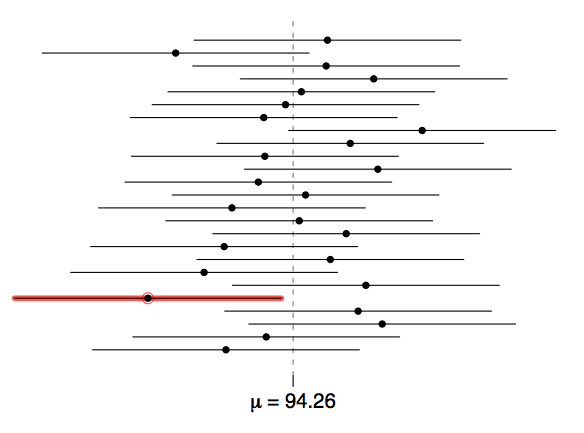
\includegraphics[scale=0.4]{ConfInt.png}
  \end{center}
}

\frame{
  \frametitle{Nominal Data}
  {\Large{What kind of population parameters could we be interested in for nominal data?}}
}



\end{document}
